\documentclass[letterpaper,10pt]{article}

\usepackage{enumitem}
\usepackage{titling}
\usepackage{listings}
\usepackage{url}
\usepackage{hyperref}
\usepackage{setspace}
\usepackage{subfig}
\usepackage{sectsty}
\usepackage{pdfpages}
\usepackage{colortbl}
\usepackage{multirow}
\usepackage{multicol}
\usepackage{relsize}
\usepackage{amsmath}
\usepackage{wasysym}
\usepackage{fancyvrb}
\usepackage[yyyymmdd]{datetime}
\usepackage{amsmath,amssymb,amsthm,graphicx,xspace}
\usepackage[titlenotnumbered,noend,noline]{algorithm2e}
\usepackage[compact]{titlesec}
\usepackage{XCharter}
\usepackage[T1]{fontenc}
\usepackage[scaled]{beramono}
\usepackage[normalem]{ulem}
\usepackage{booktabs}
\usepackage{tikz}
\usetikzlibrary{arrows,automata,shapes,trees,matrix,chains,scopes,positioning,calc}
\tikzstyle{block} = [rectangle, draw, fill=blue!20,
text width=2.5em, text centered, rounded corners, minimum height=2em]
\tikzstyle{bw} = [rectangle, draw, fill=blue!20,
text width=4em, text centered, rounded corners, minimum height=2em]

\definecolor{namerow}{cmyk}{.40,.40,.40,.40}
\definecolor{namecol}{cmyk}{.40,.40,.40,.40}
\renewcommand{\dateseparator}{-}

\let\LaTeXtitle\title
\renewcommand{\title}[1]{\LaTeXtitle{\textsf{#1}}}

\lstset{basicstyle=\footnotesize\ttfamily,breaklines=true}

\newcommand{\handout}[5]{
	\noindent
	\begin{center}
		\framebox{
			\vbox{
				\hbox to 5.78in { {\bf SE 350: Operating Systems } \hfill #2 }
				\vspace{4mm}
				\hbox to 5.78in { {\Large \hfill #4  \hfill} }
				\vspace{2mm}
				\hbox to 5.78in { {\em #3 \hfill \today} }
			}
		}
	\end{center}
	\vspace*{4mm}
}

\newcommand{\lecture}[3]{\handout{#1}{#2}{#3}{Lecture#1}}
\newcommand{\tuple}[1]{\ensuremath{\left\langle #1 \right\rangle}\xspace}

\newcommand{\Rplus}{\protect\hspace{-.1em}\protect\raisebox{.35ex}{\smaller{\smaller\textbf{+}}}}
\newcommand{\Cpp}{\mbox{C\Rplus\Rplus}\xspace}


\addtolength{\oddsidemargin}{-1.000in}
\addtolength{\evensidemargin}{-0.500in}
\addtolength{\textwidth}{2.0in}
\addtolength{\topmargin}{-1.000in}
\addtolength{\textheight}{1.75in}
\addtolength{\parskip}{\baselineskip}
\setlength{\parindent}{0in}
\renewcommand{\baselinestretch}{1.5}
\newcommand{\term}{Winter 2023}
\newcommand{\termnumeric}{1231}

\singlespace


\begin{document}

\lecture{ 23 --- Caching }{\term}{Jeff Zarnett}

\section*{Caching}
\begin{quote}
\textit{Caching is very... hit and miss.}
\end{quote}


Caching is very important in computing, and not just memory. We examine the idea of caching in the context of memory, but it is applicable any time there is a large resource that is divided into pieces, some of which are used more often than others. Caching provides a significant benefit in some circumstances and not useful in others (hence ``hit and miss''). The goal of caching is to speed up operations. It is desirable to read information from cache, when possible, because it takes less time to get data from cache to the CPU than from main memory to the CPU. CPUs are a lot faster than memory and it is best if we do not keep them waiting.

Caches do not have to operate on pages; they can operate on anything, but they are typically blocks of a given size. An entry in a cache is often called a \textit{line}. We will assume for the balance of this discussion that a cache line maps nicely to a page.

As discussed, the CPU generates a memory address for a read or write operation. The address will be mapped to a page. Ideally, the page is found in the cache, because that would be faster. If the requested page is, in fact,  in the cache, we call that a cache \textit{hit}. If the page is not found in the cache, it is considered a cache \textit{miss}. In case of a miss, we must load the page from memory, a comparatively slow operation. A page miss is also called a \textit{page fault}. The percentage of the time that a page is found in the cache is called the \textit{hit ratio}, because it is how often we have a cache hit. We can calculate the effective access time if we have a good estimate of the hit ratio (which is not overly difficult to obtain) and some measurements of how long it takes to load data from the cache and how long from memory. The effective access time is therefore computed as:

\begin{center}
Effective Access Time = $h \times t_{c} + (1-h) \times t_{m}$
\end{center}

Where $h$ is the hit ratio, $t_{c}$ is the time required to load a page from cache, and $t_{m}$ is the time to load a page from memory. Of course, we would like the hit ratio to be as high as possible. 

Caches have limited size, because faster caches are more expensive. With infinite money we might put everything in registers, but that is rather unrealistic. Caches for memory are very often multileveled; Intel 64-bit CPUs tend to have L1, L2, and L3 caches. L1 is the smallest and L3 is the largest. Obviously, the effective access time formula needs to be updated and expanded, when we have multiple levels of cache with different access times and hit rates. See the diagram below:

\begin{center}
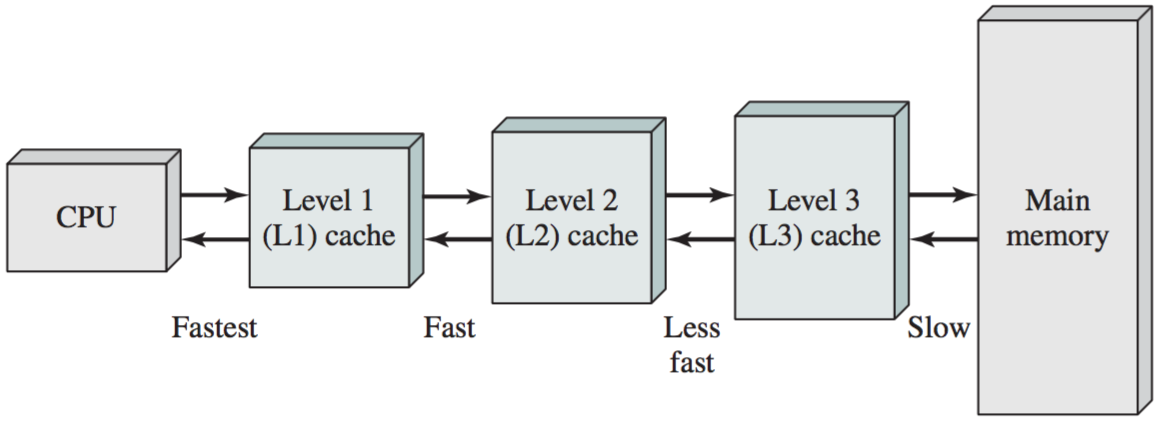
\includegraphics[width=0.6\textwidth]{images/caches.png}\\
Three levels of cache between the CPU and main memory~\cite{osi}.
\end{center}

If we have a miss in the L1 cache, the L2 cache is checked. If the L2 cache contains the desired page, it will be copied to the L1 cache and sent to the CPU. If it is not in L2, then L3 is checked. If it is not there either, it is in main memory and will be retrieved from there and copied to the in-between levels on its way to the CPU. Because caches have limited size, we have to manage this storage carefully.

\subsection*{Page Replacement Algorithms}
Whenever a page fault occurs, the operating system needs to choose which page to \textit{evict} from (kick out of) the cache to make space for the new one. This assumes that the cache is full, which it likely is except at system startup. We could, of course, just select a random page, but we should do this task more intelligently, if we can.

To make an intelligent decision about what sort of strategy to choose, we need to know a few things about how data is accessed in a system. A few observations from~\cite{mte241}:

\begin{enumerate}
	\item A rule of thumb in software engineering is that 10\% of the source code will be executed 90\% of the time. This is a variant on the Pareto Principle, also known as the 80/20 rule\footnote{Note that the 80/20 rule is not always applicable. For example, studying 20\% of the course material is unlikely to earn you 80\% of the marks on the exam.}. This may seem sensible to you given that code has a lot of handling of special cases and rarely used operations.
	\item The principle of \textit{temporal locality}: a memory location that has been recently accessed is likely to be accessed again in the future. 
	\item The principle of \textit{spatial locality}: a memory location near one that has recently been accessed is likely to be accessed again in the future.
\end{enumerate}

An example of code that would involve both spatial and temporal locality might be a function that sums up all the values of an array. The sum variable is accessed repeatedly, and the fact that it was recently accessed means it is likely to be accessed again soon. The array being accessed at index $i$ now means it is likely that the array at index $i+1$ is likely to be accessed soon.

If a page has been altered in cache, then that change has to be written to main memory at some point. It can be done immediately when the page is changed, or it can be done when the page is evicted from the cache. The second option means fewer main memory accesses, if a page is written to multiple times before it is sent to main memory. If that memory is shared, however, between multiple processors or an I/O device, then the delay in updating main memory may be intolerable. If a page has not been modified in cache, it can simply be overwritten. If all other factors are equal, we should replace a page that has not been modified, as the work to write it out to memory need not be done.

\paragraph{The Optimal Algorithm.}
The optimal page replacement algorithm is fairly simple: replace the page that will be used most distantly in the future. For each page, make a determination about how many instructions in the future that page will be accessed. The selected page is the one with the highest value.

Unfortunately, there is a glaring flaw in this algorithm: it is impossible to implement. It requires clairvoyance (seeing into the future), and at least as far as I know, nobody has invented a way to do so reliably\footnote{Recall the joke ``Why do you never see the newspaper headline that a psychic has won the lottery?''}. The program and operating system have no real way of knowing which pages will be used in the future.

As it is unimplementable, it is mostly a benchmark against which other algorithms can be compared. If we know that a given algorithm is, say 1\% less efficient than the hypothetical optimal algorithm, then no matter how much we improve that algorithm, the best performance increase we can get is 1\%~\cite{mos}.

\paragraph{Not-Recently-Used.}
Operating systems may collect page usage statistics. If so, computers may have two status bits associated with each page, called $R$ and $M$. The $R$ bit is set when a page is referenced (either read or written) and the $M$ bit is set when the page is written to (modified). Once a bit is set, it remains so until the OS changes its value. The $R$ and $M$ bits can used to build a paging algorithm as follows~\cite{mos}:

Initially, $R$ and $M$ are 0. Periodically, the $R$ bit is cleared to distinguish pages that have not been recently referenced. This may happen every clock interrupt, for example. When a replacement needs to take place, the operating system will examine all the pages and sort them into four buckets based on the $R$ and $M$ bits, in ascending order of precedence:

\begin{enumerate}
	\item Not referenced, not modified.
	\item Not referenced, modified.
	\item Referenced, not modified.
	\item Referenced, modified.
\end{enumerate}

The OS will prefer to remove a page from the lowest-numbered class, when possible. This NRU algorithm is fairly easy to understand and may provide adequate performance.

\paragraph{First-In-First-Out.}
First-In-First-Out is quite easy to understand and implement; the idea is some sort of temporal locality. If there are $N$ frames, keep a counter that points to the frame that is to be replaced (the counter ranges from $0$ to $N-1$). Whenever a page needs to be replaced, replace the page at the counter index and increment the counter, wrapping around to 0 where necessary.

Some of the time this strategy works: if a page is not going to be referenced again (or at least, for a very long time), it is a good choice to get rid of. Often times, however, the same page is referenced repeatedly, and this algorithm does not take that into account. If a page is referenced often, we want to keep it in memory, not evict it just because it has been in the cache the longest. So FIFO is probably not the best choice.

\paragraph{A Second Chance (the Clock Algorithm).} 
To improve on the FIFO algorithm, suppose we give pages a ``second chance'' based on whether or not the $R$ bit is set. If the oldest page has not been used recently (the $R$ bit is not set), then the oldest page is removed. If the oldest page has recently been referenced, the R bit is cleared. The search then goes backwards (to the next-oldest page) and repeats the procedure. This happens until a page is removed. Because the algorithm clears the $R$ bit as it goes, even if all pages have recently been referenced, eventually a  page will be selected and evicted. Thus the algorithm will eventually terminate. The index is updated whenever this happens so a page that got a second chance is not the ``oldest'' anymore. In some textbooks this is called the Clock replacement algorithm because we can think of the cache as a circular buffer and the current oldest page as being pointed to by the hand of the clock~\cite{mos}. 

This addresses the problem of a page that is frequently used eventually becoming the oldest and being evicted, only to be brought back into memory again immediately afterwards.

\paragraph{Least Recently Used (LRU).}
The least recently used (LRU) algorithm means the page that is to be replaced is the one that has been accessed most distantly in the past. You might consider time stamps and searching a list, but because there are only two operations, it need not be that complex. When a page in the cache is accessed, move that page to the back of the list. When a page is not found in cache, the page at the front of the list is removed and the new page is put at the back of the list. This requires nothing more than a cyclic doubly-linked list. Both operations can be performed in $\Theta(1)$ time~\cite{mte241}.

\begin{center}
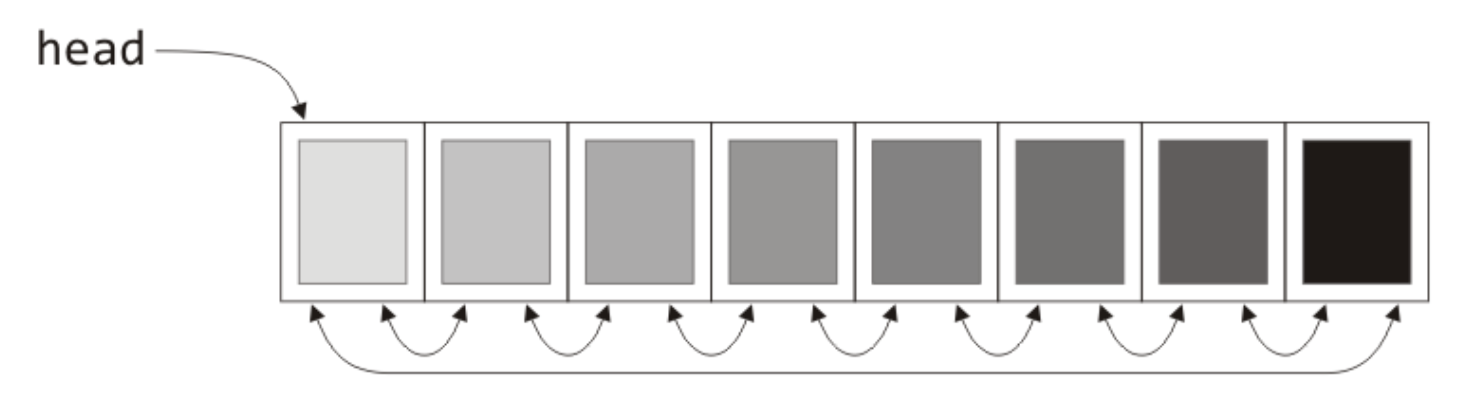
\includegraphics[width=0.7\textwidth]{images/lru-linkedlist.png}\\
A cyclic, doubly-linked list in which the \texttt{head} pointer indicates the least recently used page~\cite{mte241}.
\end{center}

\paragraph{Not Frequently Used (NFU).}
The not frequently used (NFU) algorithm is similar to the LRU approach, but can be implemented in software rather than relying on hardware support that may not be present. Each page gets an associated software counter, which starts at 0. Whenever the $R$ bit would have been updated to 1, 1 is added to the counter. When a page is to be replaced, the page with the lowest counter value is the one that is replaced~\cite{mos}. 

It may occur to you that this solution has a problem: like an elephant, it never forgets and counters can never decrease. A page that was accessed very frequently at the start of the program will accumulate a high counter value early on, and therefore might never be evicted, even though it is not needed again. What we need is a way for the count to decline over time. 

The solution is called \textit{aging}: counters are shifted to the right by 1 bit before the 1 is added; and instead of adding 1 (which increments the rightmost bit), set the leftmost bit to 1. Now we have a bit array of byte size (no need for a 4-byte integer, most likely). Thus, a page that has not been referenced in a while has its value decrease over time. The page replacement algorithm still evicts the lowest value page when it is time to replace a page. We lose a certain amount of precision compared to the LRU approach: if pages $a$ and $b$ both have patterns of \texttt{00000001} we know they were both last accessed 8 cycles ago, but all history before that point is lost. Which page between $a$ and $b$ was least recently used is unknown~\cite{mos}. 

\paragraph{Pre-Paging.}
Thus far all of our strategies for putting things in the cache have been ``on-demand'': it is only when a page is needed and not found in the cache that a page is loaded into the cache. Suppose instead that the operating system takes some steps to guess about what pages might be needed next, based on the principle of temporal or spatial locality. This might reduce the amount of time spent waiting for a page in the future.

Predicting which pages are likely to be used in the near future is, indeed, a matter of clairvoyance. There exist various techniques to determine the likely pages to be used frequently (called the ``working set''), but they are complex and will not be examined further right now.

A situation in which pre-paging might be useful is when a program is started or swapped into memory. Technically, no pages of the process need to be loaded into the cache to start with; we can simply suffer through a whole bunch of page faults. This is rather slow; it might be better to load multiple pages into the cache to start with, though this will of course require some guesses about what pages will be needed~\cite{mos}.

\subsection*{Choosing an Algorithm}
Consider the following table that gives a quick overview of the algorithms we have discussed:

\begin{center}
\begin{tabular}{l|l}
	\textbf{Algorithm} & \textbf{Comment} \\ \hline
	Optimal & Impossible to implement, but a benchmark to compare against\\
	Not Recently Used &  Not very good performance \\
	First In First Out & Highly suboptimal \\
	Second Chance & Much better than FIFO, but just adequate \\
	Least Recently Used & Best performer, difficult to implement? \\
	Not Frequently Used & Approximation of LRU \\
	NFU + Aging & Better approximation of LRU\\
\end{tabular}
\end{center}

If hardware is available to support it, the LRU algorithm is the best. If not, the NFU + Aging scheme is the next best thing we can implement. Unless there is a specific reason to choose one of the other algorithms, LRU is very likely to be the algorithm selected.

\subsection*{Local and Global Algorithms}
When a process switch occurs, we could dump the entire cache to make way for the next process to run, but this is most likely unnecessary work. If a process $P_{1}$ is suspended now, $P_{2}$ may run for a while and then $P_{1}$ runs again; it may be that when $P_{1}$ starts again, some of its pages are still in the cache and do not need to be loaded again. If $P_{2}$ did replace all the cache lines, then $P_{1}$ will have to load them all in again, but that is the worst case scenario. So we may have multiple processes with pages in the cache at a given time.

Another important consideration in the page replacement algorithm is whether that algorithm should care about which process the page belongs to or not. Suppose we are using the LRU algorithm. If process $P_{1}$ has a page fault, do we replace the least recently used page in all the cache (global replacement)? Or do we replace the least recently used page in the cache that belongs to $P_{1}$ (local replacement)?

Of course, different levels of cache might have different strategies: if the L1 cache is 16~KB and pages are 4~KB, there can be 4 pages in the L1 cache, so global replacement probably makes sense there. If L2 cache is 256~KB there are 64 pages and maybe local replacement makes sense there, but even 64 pages is fairly small. When caches are somewhat larger, however, things may be a bit more interesting.

Local algorithms give each process some (roughly) fixed number of pages in the cache. Global algorithms dynamically allocate cache space to different programs based on their needs, so the number of pages in the cache for each process can vary over time. 

According to~\cite{mos}, global algorithms work better, especially when processes' memory needs change over time. If the local algorithm is used, we may be wasting some of the space in the cache for a process that does not really need it. 

Suppose we have a sufficiently large cache, and a dynamic allocation (global algorithm) with some intelligence to keep any process from having too many or too few pages in the cache. To manage the complexity of how much of the cache should be allocated to a particular process, we might wish to keep track of the number of page faults with a measure called the \textit{page fault frequency} or PFF. In simplest terms, the PFF is the guide for telling whether a given process has too few, too many, approximately the right number of pages. 

If the PFF is above some upper threshold, that indicates that more cache space is needed for that process. If the PFF is below some lower threshold, it suggests that the process has too much cache space allocated and could stand to part with some.

PFF relies on an assumption: that the page replacement algorithm has the property that fewer page faults will occur if a process has more pages assigned. This is the case for the LRU algorithm, but not necessarily true for the FIFO approach~\cite{mte241}.


\bibliographystyle{alphaurl}
\bibliography{350}


\end{document}
